
\section{Auswertung}
\subsection{Bestimmung der Reichweite von $\alpha$-Strahlung}
In Tabelle \ref{tab:2cm} und \ref{tab:15cm} sind die gemessenen Werte für einen
Abstand vo 2\,cm  und 1,5\,cm aufgetragen.
Die Energien ergeben sich durch den gemessenen Channel.
bei 0\,bar wird dieser auf 4\,MeV gesetzt.
Die effektive Länge x wird mit Formel (\ref{eqn:eff}) bestimmt.

\begin{table}
  \centering
  \caption{Messwerte für einen Abstand von 2\,cm}
  \label{tab:2cm}
  \begin{tabular}{c c c c c c c}
    \toprule
    p/mbar & Channel & plses detected & Counts & Energie/MeV & x/cm\\
    \midrule
    0   & 678 & 73686 & 310 & 4,00 & 0,00 \\
    50  & 661 & 74263 & 315 & 3,90 & 0,10 \\
    100 & 590 & 65991 & 355 & 3,48 & 0,20 \\
    150 & 574 & 63764 & 348 & 3,39 & 0,30 \\
    200 & 556 & 61555 & 367 & 3,28 & 0,39 \\
    250 & 531 & 59580 & 412 & 3,13 & 0,49 \\
    300 & 523 & 56438 & 401 & 3,09 & 0,59 \\
    350 & 559 & 65994 & 414 & 3,30 & 0,69 \\
    400 & 534 & 65102 & 433 & 3,15 & 0,79 \\
    450 & 523 & 61636 & 430 & 3,09 & 0,89 \\
    500 & 502 & 58166 & 444 & 2,96 & 0,99 \\
    550 & 447 & 29551 & 434 & 2,64 & 1,09 \\
    600 & 443 & 23408 & 424 & 2,61 & 1,18 \\
    650 & 441 & 39064 & 492 & 2,60 & 1,28 \\
    700 & 438 & 31817 & 515 & 2,58 & 1,38 \\
    750 & 438 & 22589 & 413 & 2,58 & 1,48 \\
    800 & 439 & 16150 & 374 & 2,59 & 1,58 \\
    850 & 435 & 6415  & 221 & 2,57 & 1,68 \\
    900 & 463 & 8408  & 267 & 2,73 & 1,78 \\
    950 & 434 & 1681  & 71  & 2,56 & 1,88 \\
    1000& 435 & 440   & 25  & 2,57 & 1,97 \\
    \bottomrule
  \end{tabular}
\end{table}

\begin{table}
  \centering
  \caption{Messwerte für einen Abstand von 1,5\,cm}
  \label{tab:15cm}
  \begin{tabular}{c c c c c c}
    \toprule
    p/mbar & Channel & plses detected & Counts & Energie/MeV & x/cm\\
    \midrule
    50  & 635 & 94734 & 452 & 4,00 & 0,07\\
    100 & 631 & 93282 & 447 & 3,97 & 0,15\\
    150 & 611 & 92420 & 512 & 3,85 & 0,22\\
    200 & 596 & 90285 & 533 & 3,75 & 0,30\\
    250 & 577 & 88404 & 485 & 3,63 & 0,37\\
    300 & 567 & 87319 & 519 & 3,57 & 0,44\\
    350 & 552 & 84497 & 541 & 3,48 & 0,52\\
    400 & 528 & 83263 & 541 & 3,33 & 0,59\\
    450 & 519 & 80395 & 556 & 3,27 & 0,67\\
    500 & 510 & 76957 & 580 & 3,21 & 0,74\\
    550 & 495 & 73038 & 630 & 3,12 & 0,81\\
    600 & 479 & 67618 & 612 & 3,02 & 0,89\\
    650 & 456 & 61821 & 663 & 2,87 & 0,96\\
    700 & 446 & 55155 & 655 & 2,81 & 1,04\\
    750 & 440 & 46731 & 748 & 2,77 & 1,11\\
    800 & 440 & 41832 & 703 & 2,77 & 1,18\\
    850 & 440 & 29176 & 644 & 2,77 & 1,26\\
    900 & 440 & 22214 & 572 & 2,77 & 1,33\\
    950 & 439 & 17223 & 466 & 2,77 & 1,41\\
    1000& 438 & 11192 & 349 & 2,76 & 1,48\\
    \bottomrule
  \end{tabular}
\end{table}

\begin{figure}[H]
\centering
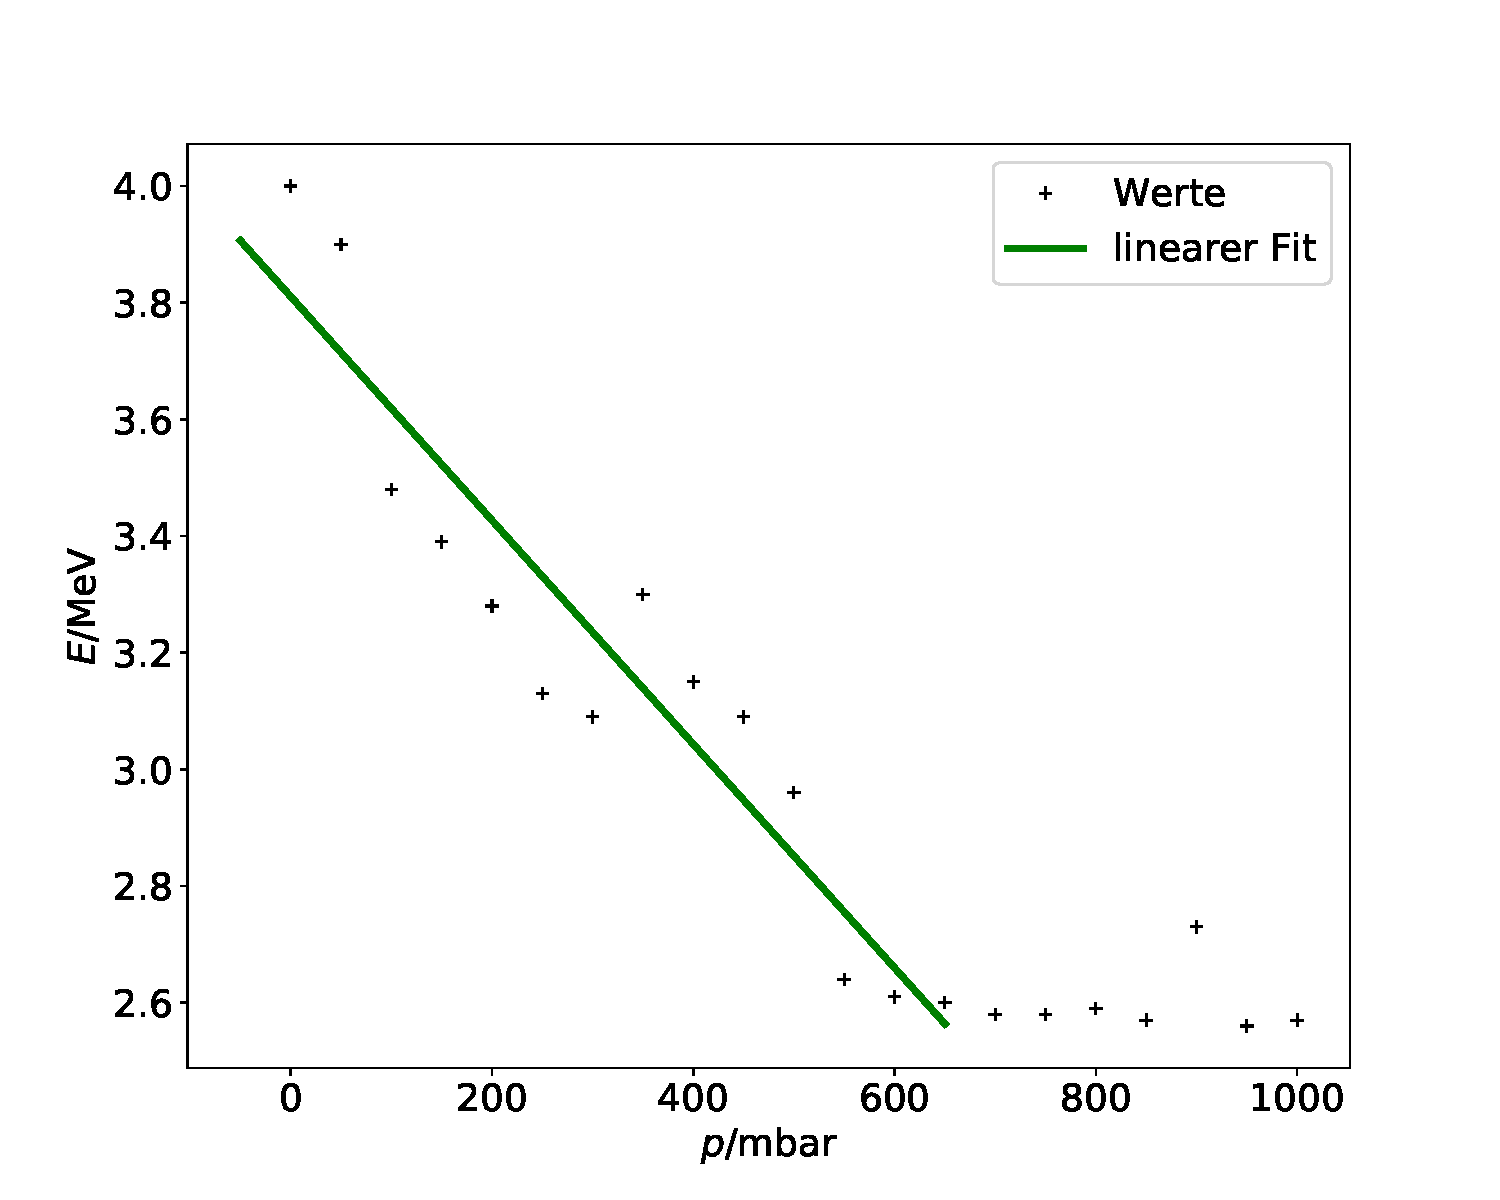
\includegraphics[width=\textwidth]{ep2.pdf}
\caption{Energien der $\alpha$-Teilchen in Abhängigkeit des Drucks in einem Abstand von 2\,cm}
\label{fig:ep2}
\end{figure}

\begin{figure}[H]
\centering
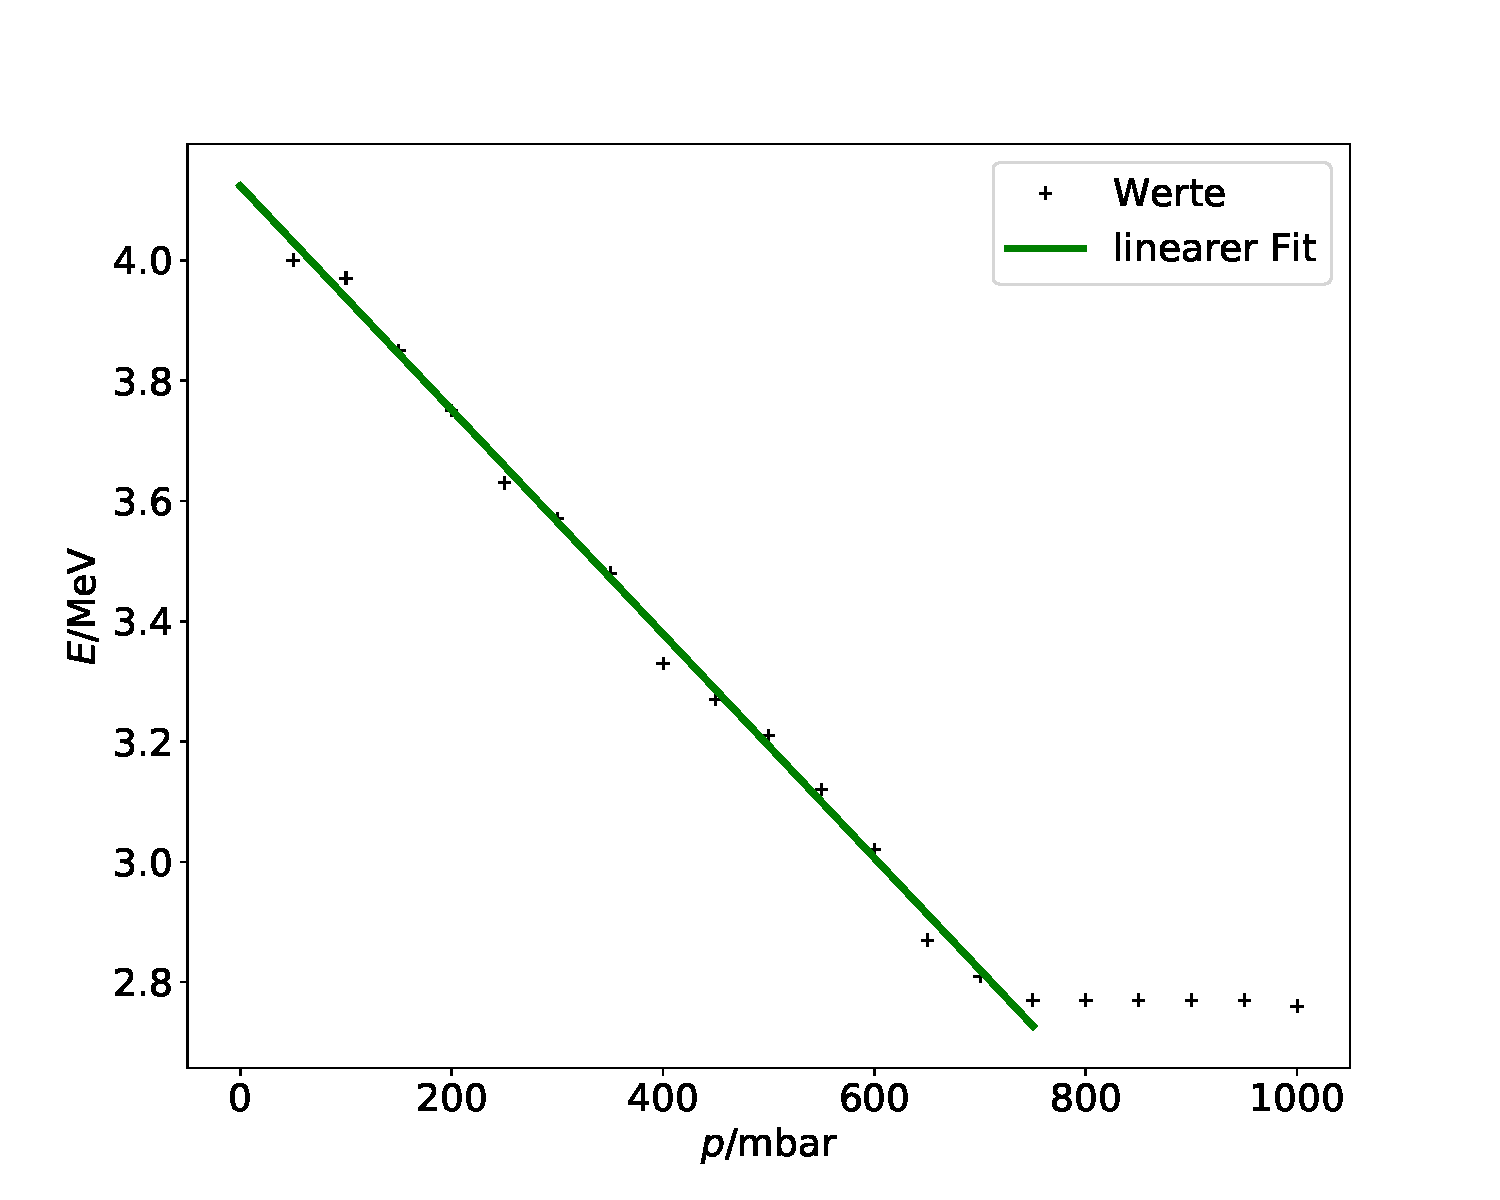
\includegraphics[width=\textwidth]{ep15.pdf}
\caption{Energien der $\alpha$-Teilchen in Abhängigkeit des Drucks in einem Abstand von 1,5\,cm}
\label{fig:ep15}
\end{figure}

Die lineare Regregression wurde  jeweils mit
\begin{align*}
  E(p)= a\cdot p +b
\end{align*}
durchgeführt.
Die daraus resultierenden Parameter lauten
\begin{align*}
  a_{2}  &= (-0,0019\pm 0,0002)\, \mathrm{\frac{MeV}{mbar}} & a_{1,5} &=(-0,00186\pm 0,00004)\, \mathrm{\frac{MeV}{mbar}} \\
  b_2 &= (3,81\pm0,08)\,\mathrm{MeV} & b_{1,5} &=(4,12\pm0,02)\, \mathrm{MeV}
\end{align*}

Zur Bestimmung der mittleren Reichweite wird die Zählrate gegen die effektive Länge aufgetragen.
Dies ist in den Abbildungen \ref{fig:mreich1} und \ref{fig:mreich2} zu sehen.

\begin{figure}[H]
\centering
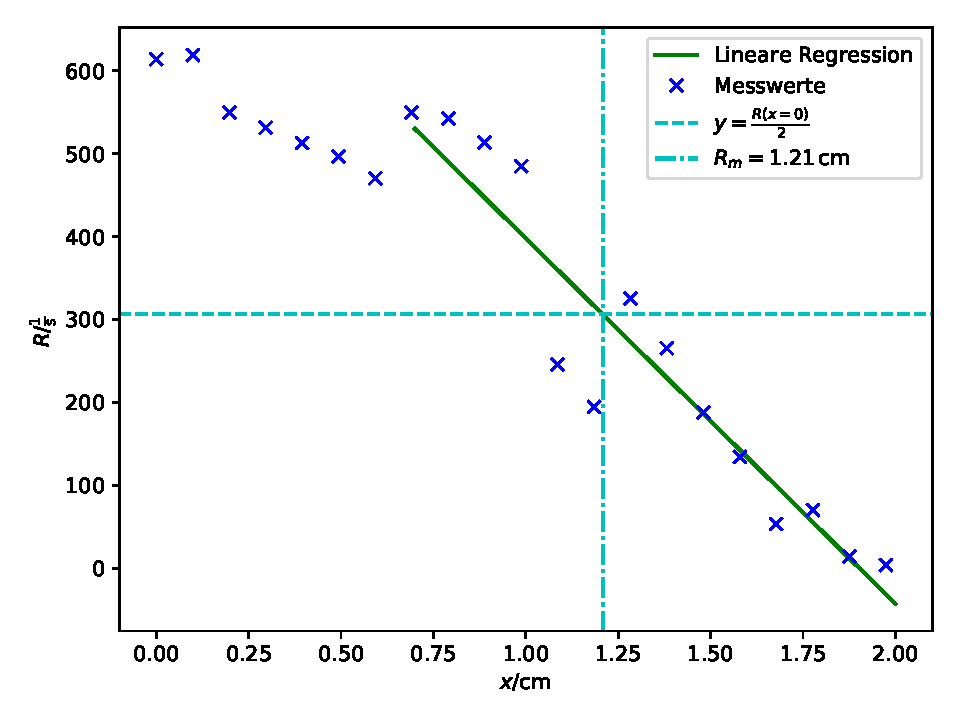
\includegraphics[width=\textwidth]{mreich2.pdf}
\caption{Zählrate der $\alpha$-Teilchen in Abhängigkeit der effektiven Länge in einem Abstand von 2\,cm}
\label{fig:mreich2}
\end{figure}

\begin{figure}[H]
\centering
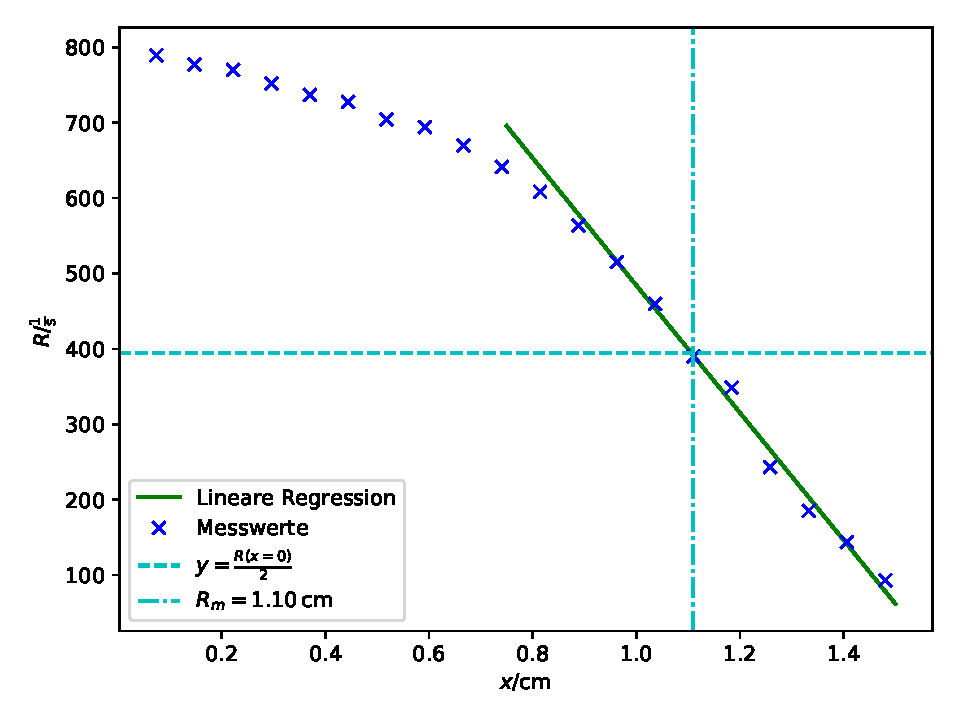
\includegraphics[width=\textwidth]{mreich1.pdf}
\caption{Zählrate der $\alpha$-Teilchen in Abhängigkeit der effektiven Länge in einem Abstand von 1,5\,cm}
\label{fig:mreich1}
\end{figure}

Die lineare Regression wurde mit
\begin{equation*}
R(x) = a\cdot x +b
\end{equation*}
durchgeführt.
Die ermittelten Parameter lauten
\begin{align*}
  a_2&=(-4,4\pm0,6)\cdot10^2 \,\mathrm{s^{-1}cm^{-1}}& a_{1,5}&= (-854\pm33)\,\mathrm{s^{-1}cm^{-1}}\\
  b_2&=(8,4\pm0,8)\cdot10^2\,\mathrm{s^{-1}} & b_{1,5}&= (1,33\pm0,04)\cdot 10^3\,\mathrm{s^{-1}}
\end{align*}
Die zugehörigen Energien werden mit Hilfe der Formel (\ref{eqn:Rm}) bestimmt.
Sie lauten:
\begin{align*}
  E_{2} &= 2,48\,\mathrm{MeV}\\
  E_{1,5} &= 2,34\,\mathrm{MeV}
\end{align*}
Nun wird der Energieverlust $-\frac{dE}{dx}$ bestimmt in dem die Energie
als Funktion der effektiven Länge aufgetragen wird.
Dies ist in Abbildung \ref{fig:dedx} zu sehen.
\begin{figure}[H]
\centering
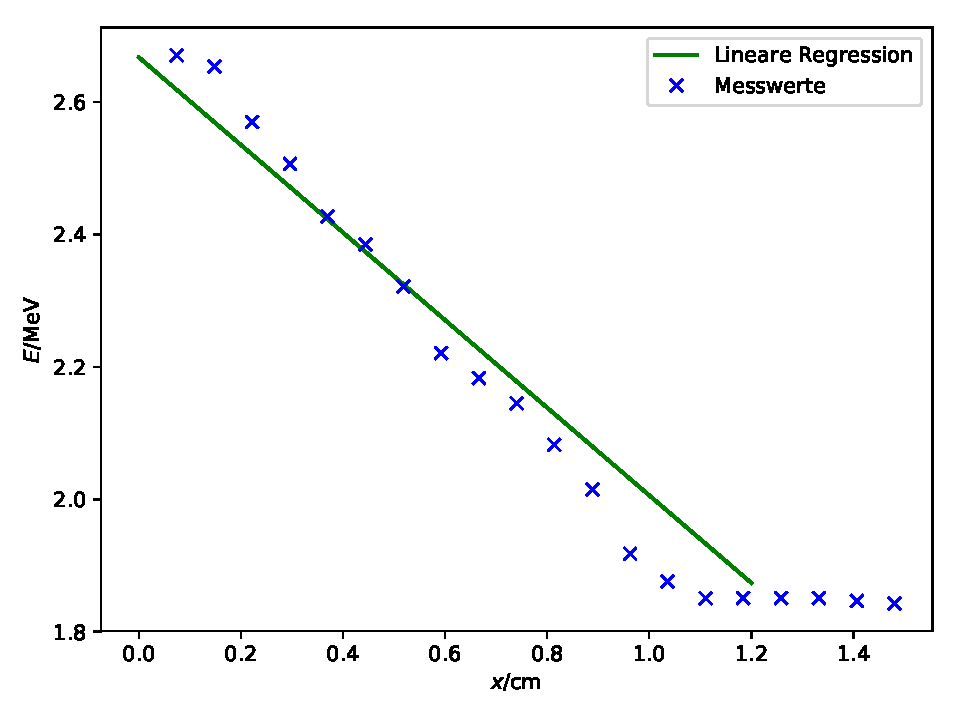
\includegraphics[width=\textwidth]{Messung1c.pdf}
\caption{Energieverlust}
\label{fig:dedx}
\end{figure}
Die lineare Regression wurde mit
\begin{equation*}
  E(x)=ex+E_0
\end{equation*}
durchgeführt.
Die Parameter betragen
\begin{align*}
  E_0 &= (2,67\pm 0,03)\, \mathrm{MeV}\\
  -\frac{dE}{dx}= e &= (0,66\pm 0,4)\,\mathrm{\frac{MeV}{cm}}
\end{align*}
\subsection{Statistik des radioaktiven Zerfalls}
Zunächst wird der Mittelwert aus den gemessenen Werten bestimmt.
Dieser beträgt $\bar{N}= 7481,72$ und wurde mit
\begin{equation*}
  \bar{N}= \frac{\sum (N)}{n}
\end{equation*}
bestimmt.
Dabei ist n=103
Die Abweichung wird mit
\begin{equation*}
  \sigma = \sqrt{\frac{\sum(N-\bar{N})^2}{n-1}}
\end{equation*}
bestimmt und beträgt $\sigma = 264,45$.\\
In Abbildung \ref{fig:statistik} sind die gemessenen Werte aus Tabelle \ref{tab:e}
sowie die Normal- un Poissonverteilung als Histogramm aufgetragen.
\begin{figure}[H]
\centering
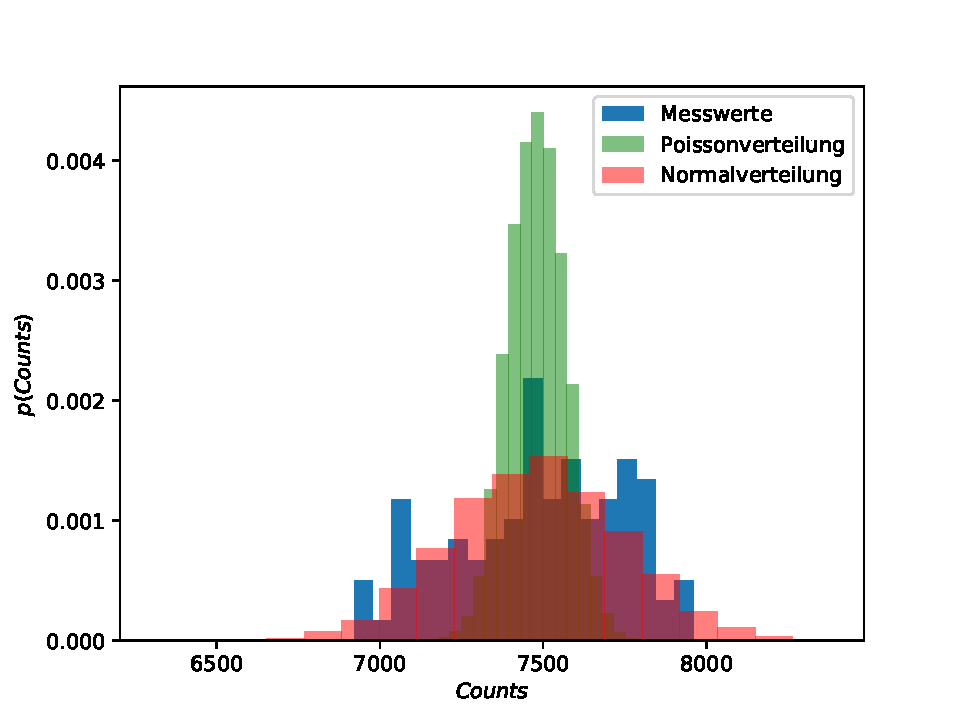
\includegraphics[width=\textwidth]{Statistik.pdf}
\caption{Histogramm der Messwerte mit der Poissonverteilung und der Normalverteilung}
\label{fig:statistik}
\end{figure}

\begin{table}
  \centering
  \caption{gemessene Counts pro 10\,s}
  \label{tab:e}
  \begin{tabular}{c c|c c|c c|c c|c c}
    \toprule
    Messung & Counts & Messung & Counts & Messung & Counts & Messung & Counts & Messung & Counts \\
    \midrule
    1  & 7569 & 26 & 7060 & 51 & 7500 & 76 & 7799 & 101 & 7528 \\
    2  & 7186 & 27 & 7260 & 52 & 7483 & 77 & 7838 & 102 & 7058 \\
    3  & 7807 & 28 & 7049 & 53 & 7378 & 78 & 7724 & 103 & 7188 \\
    4  & 7696 & 29 & 7838 & 54 & 7106 & 79 & 7547 & & \\
    5  & 7771 & 30 & 7126 & 55 & 7566 & 80 & 7774 & & \\
    6  & 7874 & 31 & 7050 & 56 & 7401 & 81 & 7293 & & \\
    7  & 7750 & 32 & 6975 & 57 & 7575 & 82 & 7038 & & \\
    8  & 7836 & 33 & 7453 & 58 & 7729 & 83 & 7658 & & \\
    9  & 7649 & 34 & 7540 & 59 & 7536 & 84 & 7238 & & \\
    10 & 7283 & 35 & 7478 & 60 & 7717 & 85 & 7185 & & \\
    11 & 7786 & 36 & 7450 & 61 & 7583 & 86 & 7337 & & \\
    12 & 7771 & 37 & 7335 & 62 & 7713 & 87 & 6921 & & \\
    13 & 7568 & 38 & 7492 & 63 & 7434 & 88 & 6990 & & \\
    14 & 7299 & 39 & 7492 & 64 & 7625 & 89 & 7110 & & \\
    15 & 7960 & 40 & 7419 & 65 & 7743 & 90 & 7369 & & \\
    16 & 7590 & 41 & 7506 & 66 & 7466 & 91 & 7039 & & \\
    17 & 7213 & 42 & 7675 & 67 & 7927 & 92 & 7444 & & \\
    18 & 7621 & 43 & 7549 & 68 & 7229 & 93 & 7402 & & \\
    19 & 7106 & 44 & 7335 & 69 & 7272 & 94 & 7811 & & \\
    20 & 7592 & 45 & 7872 & 70 & 7688 & 95 & 7449 & & \\
    21 & 6925 & 46 & 7840 & 71 & 7743 & 96 & 7402 & & \\
    22 & 7602 & 47 & 7239 & 72 & 7746 & 97 & 7811 & & \\
    23 & 7042 & 48 & 7640 & 73 & 7768 & 98 & 7449 & & \\
    24 & 7398 & 49 & 7597 & 74 & 7456 & 99 & 7177 & & \\
    25 & 7447 & 50 & 7460 & 75 & 7624 & 100& 7959 & & \\
    \bottomrule
  \end{tabular}
\end{table}

\section{Diskussion}

In diesem Versuch treten unterschiedliche Fehlerquellen auf.
Zum einen war die Einstellung des Abstandes nicht sehr genau möglich.
Zum anderen war die Einstellung des Druckes etwas schwierig.
Dies können Begründungen für die Abweichungen in Abbilung \ref{fig:ep2} sein.
Dennoch sin die Abweichungen der mittleren Reichweiten und der Enegien eher gering.
Die Reichweiten und Energien sind in Tabelle \ref{tab:4} aufgelistet.

\begin{table}
  \centering
  \caption{Zusammenfassung der Ergebnisse}
  \label{tab:4}
  \begin{tabular}{c c c}
    \toprule
    Abstand/cm & mittlere Reichweite/cm &  Energien/MeV \\
    \midrule
    1,5& 1,10 & 2,34 \\
    2 & 1,21 & 2,48 \\
    \bottomrule
  \end{tabular}
\end{table}

Das erstellte Histogramm in Abbilung \ref{fig:statistik} weist Ähnlichkeiten zwischen
den Messwerten und der Normalverteilung auf.
Zu erwarten wäre ein Zusammenhang zu der Poissonverteilung, der allerdings nicht zu erkennen ist.
Dies lässt sich darauf zurückführen, dass nicht oft genug
 und über einen ausreichend langen Zeitraum gemessen wurde.
